\chapter{Results}
\label{cha:results}

During network training track of the average score was kept from the last $\min(N_{episodes}, 140)$ and the average predicted Q-value
for each epoch. As mentioned in the above section, there were fixed parameters and environment set for every DQN architecture. One may
notice that number of steps differs for each algorithm. The reason behind it is that there was a maximum number of steps set yet
episode could have finished earlier (and usually it did)  due to agent floating into illegal space. It is clear that chosen number of
games -- 700 was insufficient to fully train the algorithm which would allow to get more detailed results about the performance.
However, due to hardware limitations it was the maximal affordable number which enabled to train four architectures in a reasonable
time. The simulation environment was getting unstable after several hours of continuous training resulting in randomly dying processes
and therefore killing the training.

For the first 20000 $\epsilon$ gradually decreased from 1 do 0.01 with step $5e^{-5}$. It was the exploration part when the scores were
not following any particular trend. The closer $\epsilon$ was decreasing to 0 the more deterministic actions became and the
exploitation part started. The minimal epsilon was not set to zero not to terminate exploration entirely, since there was always a
likelihood that agent reaches a rare unknown state which might be a valuable experience. The maximum reward for reaching the desired
point was 2450.

\section{DQN}
\label{sec:results-dqn}

The Deep Q-Network training was stable, however the network learned significantly slower that other architectures. Although Q-value on
figure \ref{fig:avg-qval-dqn} was constantly increasing, it did not project on a score which oscillated around 200 throughout the
entire exploitation training part. Note that the Q-values are scaled due to clipping of rewards (\ref{sub2:training-algo-for-deep-q-net}). The below figure shows how the score changes when the agents switches from exploration to
exploitation. When $\epsilon$ reaches its minimum, the score drops, which is the expected behaviour. At the beginning the agent only
collected experiences but took mostly random actions which had at first mostly higher values than untrained network could predict.
Throughout training steps the score started to ascend which shows that the network was learning (adjusting its weights to minimise loss
and therefore find the optimal policy $\pi^*$) but did not manage to converge.

\begin{figure}[htb]
\begin{subfigure}{.48\textwidth}
     \centering
    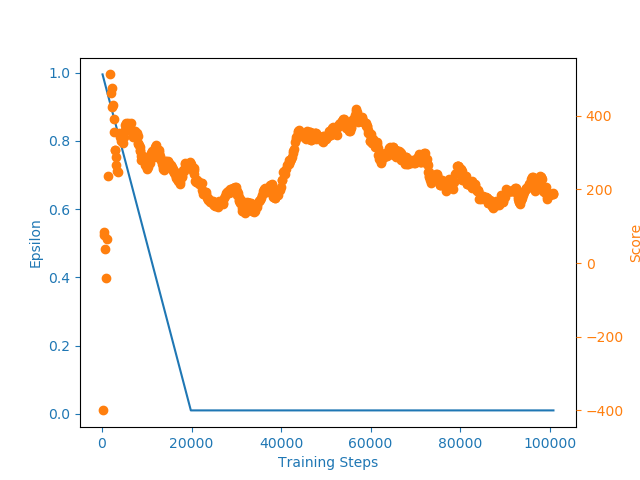
\includegraphics[width=8cm]{img/DQNAgent_WamvNavTwoSetsBuoys-v0_normal_1127_1016.png}
    \caption{Average score across training of DQN network}
    \label{fig:avg-score-dqn}   
\end{subfigure}
\begin{subfigure}{.48\textwidth}
    \centering
    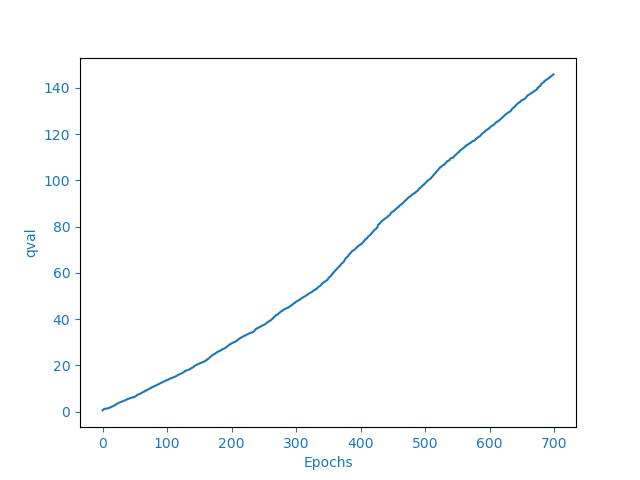
\includegraphics[width=8cm]{img/DQNAgent_WamvNavTwoSetsBuoys-v0_normal_1129_1802_qval.png}
    \caption{Average Q-value across training of DQN network}
    \label{fig:avg-qval-dqn}
\end{subfigure}
\caption{DQN training results}
\label{fig:dqn-results}
\end{figure}

\newpage

\section{Dobule DQN}
\label{sec:results-double-dqn}

The Double Q-Network performed significantly better that the predecessor. Not only did it manage to achieve four times higher score but
was also far more stable. There was one drop around 30000 step, yet the agent continued to learn more valuable actions at a given state
which eventually led to further score increase. The score of 800 is acquired when the agent reaches the most critical part of
simulation track - the curve. The network has to readjust the previously learned action patterns to changeable conditions. That is why
the score increase ratio slows down at the end. If the training was extended to greater amount of epochs the deep neural network would
have most likely adjusted its weights to overcome this obstacle. Even in the researched scenario the frequency of epochs where agent reached the
finishing line was visibly increasing towards the end of training.

The Q-value as expected is higher than in the DQN case. The underlying concept behind separating action selection from action evaluation
was to remove overestimation of the value function. Therefore correct actions were chosen more frequently.

\begin{figure}[htb]
\begin{subfigure}{.48\textwidth}
    \centering
    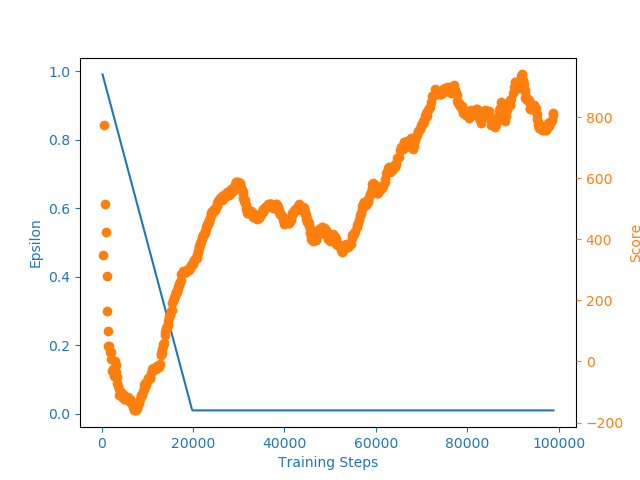
\includegraphics[width=8cm]{img/DDQNAgent_WamvNavTwoSetsBuoys-v0_normal_1126_0854.png}
    \caption{Average score across training of Double DQN network}
    \label{fig:avg-score-ddqn}
\end{subfigure}
\begin{subfigure}{.48\textwidth}
    \centering
    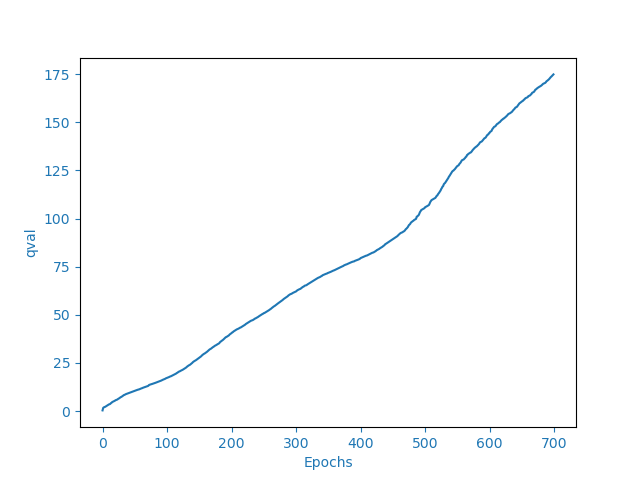
\includegraphics[width=8cm]{img/DDQNAgent_WamvNavTwoSetsBuoys-v0_normal_1126_0854_qval.png}
    \caption{Average Q-value across training of Double DQN network}
\end{subfigure}
\caption{Double DQN training results}
\label{fig:ddqn-results}
\end{figure}

\newpage

\section{Dueling DQN}
\label{sec:results-dueling-dqn}

Dueling network architecture was supposed to identify correctness of actions quicker than a standard DQN. Indeed the score started to raise faster
than in DQN and even in Double DQN. The agent chose more often the more valuable action than not, which is visible as rather stable score increase
along training with only occasional drops of low magnitude. It is worth noticing that reaching the score of 800 took 20000 less steps than for a
previous agents. The Dueling DQN learned substantially faster which is an expected outcome. For most states the exact action choice is of little
relevance as long as the agent floats towards desired point.

\begin{figure}[htb]
\begin{subfigure}{.48\textwidth}
    \centering
    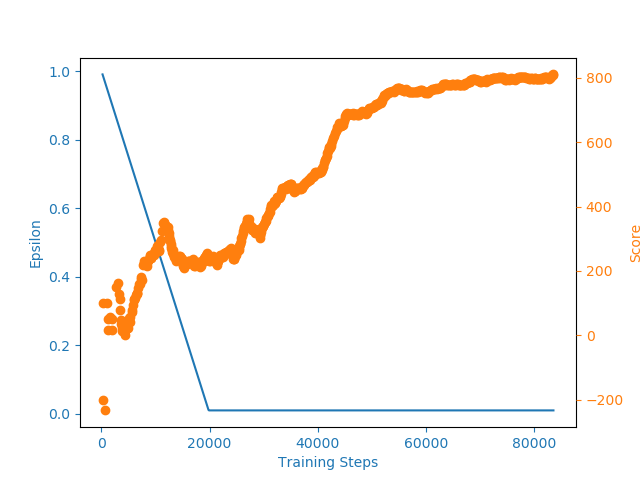
\includegraphics[width=8cm]{img/DuelingDQNAgent_WamvNavTwoSetsBuoys-v0_normal_1128_1318.png}
    \caption{Average score across training of Dueling DQN network}
    \label{fig:avg-score-dueling-dqn}
\end{subfigure}
\begin{subfigure}{.48\textwidth}
    \centering
    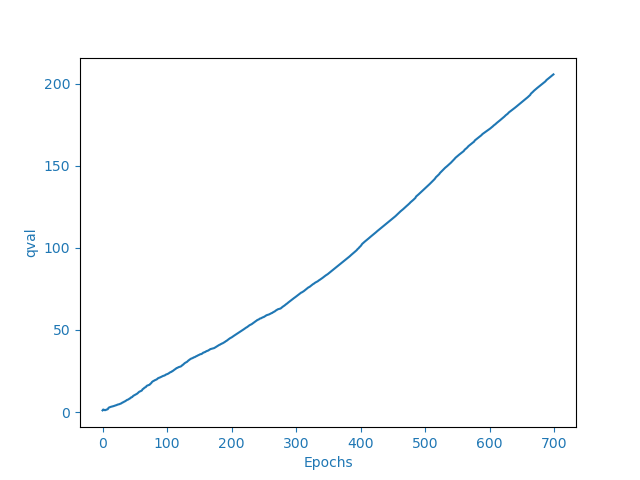
\includegraphics[width=8cm]{img/DuelingDQNAgent_WamvNavTwoSetsBuoys-v0_normal_1128_1318_qval.png}
    \caption{Average Q-value across training of Dueling DQN network}
\end{subfigure}
\caption{Dueling DQN network training results}
\label{fig:results-dueling-dqn}
\end{figure}

\section{Dueling Double DQN}
\label{sec:results-dueling-double-dqn}

It was the most robust architecture among all DQNs and there is no surprise that it outperformed the competition. The score increase
was the most stable without any significant drops. What is more, the network reached the critical point of score 800 the fastest. Although
the score flattened there the Q-value kept increasing which is a sign that the network was learning how to pass the critical point. Given more epochs for training, the Double DDQN would with every likelihood pass this threshold.

\begin{figure}[htb]
\begin{subfigure}{.48\textwidth}
    \centering
    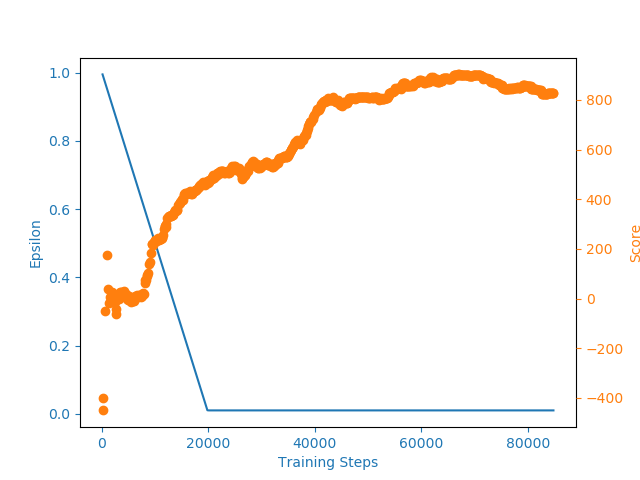
\includegraphics[width=8cm]{img/DuelingDDQNAgent_WamvNavTwoSetsBuoys-v0_normal_1125_0937.png}
    \caption{Average score across training of Dueling Double DQN}
    \label{fig:avg-score-dddqn}
\end{subfigure}
\begin{subfigure}{.48\textwidth}
    \centering
    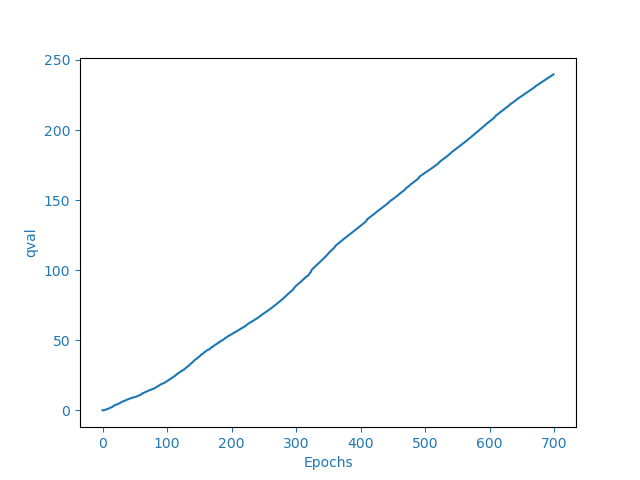
\includegraphics[width=8cm]{img/DuelingDDQNAgent_WamvNavTwoSetsBuoys-v0_normal_1125_0937_qval.png}
    \caption{Average Q-value across training of Dueling Double DQN}
\end{subfigure}
\caption{Dueling Double DQN training results}
\end{figure}

\begin{figure}[h]
    \centering
    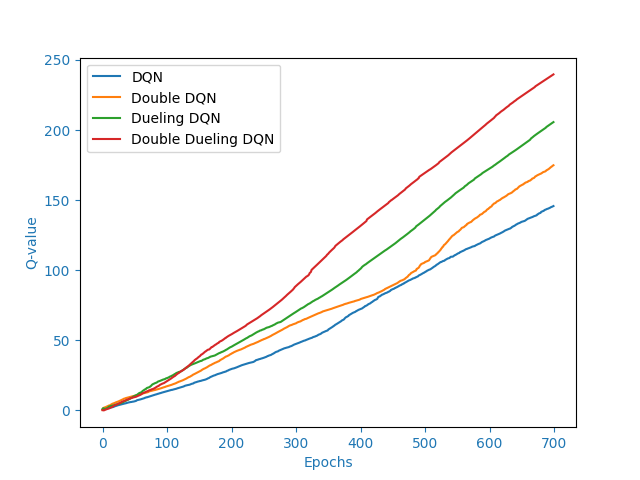
\includegraphics[width=11.5cm]{img/cumulated_qval.png}
    \caption{Comparison of average Q-values for all architectures. Note that Q-values are scaled due to clipping of rewards (see \ref{sub2:training-algo-for-deep-q-net})}
    \label{fig:results-qval-comparison}
\end{figure}